\documentclass{article}

\usepackage[utf8]{inputenc}

% Packages
\usepackage{amsmath,amssymb}
\usepackage{bm}% boldmath
\usepackage{listings} % Code block (source code) \begin{lstlisting} 
\usepackage{natbib}
\usepackage{graphicx}
\usepackage{lmodern}
\usepackage[usenames,dvipsnames,svgnames,table]{xcolor}
\usepackage[textwidth=16cm,textheight=23cm]{geometry}

%\usepackage{inconsolata} % New monospace font

% URL
\usepackage{url}
\usepackage[colorlinks=true, a4paper=true, pdfstartview=FitV, linkcolor=blue, citecolor=blue, urlcolor=blue]{hyperref}

% Figures
\usepackage[font=small, labelfont=bf]{caption}
\usepackage{subfig} % Subfigures. Uses \subfloat[captions text]{figure}

% Tables
\usepackage{booktabs}   % Allows the use of \toprule, \midrule and \bottomrule in tables for horizontal lines
\newcommand{\ra}[1]{\renewcommand{\arraystretch}{#1}} % spaces in tables

% Itemize
\usepackage{enumitem}

% Commands
%\newcommand{\code}[1]{\texttt{#1}} % \code{inline code}
\newcommand{\code}[1]{{\small\ttfamily #1}} % \code{inline code}
\newcommand{\expval}[1]{\langle #1 \rangle} %
\renewcommand{\theequation}{\arabic{section}.\arabic{equation}} % Book format equation
\renewcommand{\thefigure}{\arabic{section}.\arabic{figure}} % Book format figure
\renewcommand{\vec}[1]{{\bf #1}} % Lars likes this better than arrow

% Set page attribution
\setlength{\parindent}{0pt}


% PSTRICKS
\usepackage{pstricks,pst-node,pst-tree} % includes graph additions
\usepackage{pst-pdf} % Compiles the pictures
\usepackage{pst-node}
\usepackage{pst-plot}
\usepackage{pst-3dplot}
%\usepackage{pstricks-add,babel}




\lstset{
language=Python,                        % Code langugage
commentstyle=\color{gray},              % Comments font
basicstyle=\small\ttfamily,             % Code font, Examples: \footnotesize, \ttfamily
keywordstyle=\bfseries\color{blue},
stringstyle=\color{orange},
numbers=left,                           % Line nums position
numberstyle=\tiny,                      % Line-numbers fonts
stepnumber=1,                           % Step between two line-numbers
numbersep=5pt,                          % How far are line-numbers from code
frame=none,                             % A frame around the code
tabsize=4,                              % Default tab size
captionpos=b,                           % Caption-position = bottom
breaklines=true,                        % Automatic line breaking?
breakatwhitespace=false,                % Automatic breaks only at whitespace?
showspaces=false,                       % Dont make spaces visible
showstringspaces=false,                 % Dont make spaces visible in strings
showtabs=false,                         % Dont make tabls visible
belowskip=8pt,
morekeywords={range, xrange},
% backgroundcolor=\color{yellow}
% emph={[2]root,base}
% morekeywords={one,two,three,four,five,six,seven,eight,
}


%commentstyle=\color{gray},              % Comments font
%basicstyle=\small,                      % Code font, Examples: \footnotesize, \ttfamily



%basicstyle=\footnotesize\ttfamily,
%keywordstyle=\bfseries\color{green!40!black},
%commentstyle=\itshape\color{purple!40!black},
%identifierstyle=\color{blue},
%stringstyle=\color{orange},







% ***************************************************
% HEADER INFORMATION

\title{Diffusion Coefficient of the Lennard-Jones Fluid}
\author{Molecular Statistic}
\date{2013}

% ***************************************************

\begin{document}


% ***************************************************
% BEGIN DOCUMENT
% ***************************************************


\maketitle

\section{Introduction}

In this project we elaborate on the Molecular Dynamics (MD)
simulation we have been working on for the past weeks.
The main assignment for this project is to calculate the
diffusion coefficient $D$ of the Lennard-Jones Fluid.\\

% Image
% http://upload.wikimedia.org/wikipedia/commons/thumb/1/12/Diffusion.svg/220px-Diffusion.svg.png


%In Latin, "diffundere" means "to spread out".

\subsection{Diffusion}

Diffusion is a transport property that refers to the phenomenon
of a flow of material from one region to another,
which arises from migration of matter down a concentration gradient.
Since we are dealing with a homogeneous liquid, there is no
meaning in defining a concentration gradient.
What we are dealing with
in this simulation is {\em self-diffusion}.\\

As described by Leach\footnote{Leach section 7.6.3 p. 380}
if we can calculate the two properties
mean-square displacement (MSD)
and the velocity auto-correlation function (VACF)
we can calculate the self-diffusion coefficient $D$.\\

Quick refresh;
two equations relate the diffusion coefficient with microscopic properties.
The relation between the MSD and VACF and $D$ is as follows;

\begin{eqnarray}
    D &=& \lim_{t\rightarrow \infty} \frac{\mathrm{MSD}(t)}{6t}\\
    D &=& \frac{1}{3} \int_0^\infty \mathrm{VACF}(t) \ \ dt
\end{eqnarray}

MSD is defined as;

\begin{eqnarray}
    \mathrm{MSD}(t) = \expval{|\vec{r}(t_0 + t) - \vec{r}(t_0)|^2}
    = \frac{1}{N} \sum_{i=1}^N | \vec{r}_i(t_0 + t) - \vec{r}_i(t_0)  |^2
\end{eqnarray}

where $\expval{x}$ indicates the expected, or average, value
$N$ is the number of particles and
$\vec{r}_i(t_0 + t)$ is the position vector of particle $i$ at time $t$ away from a time origin.\\

VACF is defined as;

\begin{eqnarray}
    \mathrm{VACF}(t) = \expval{\vec{V}(t_0 + t)\cdot\vec{V}(t_0)}
    = \frac{1}{N} \sum_{i=1}^N \vec{V}_i(t_0 + t) \cdot \vec{V}_i(t_0)
\end{eqnarray}

where
$\vec{V}_i(t_0 + t)$ is the velocity vector for particle $i$ at time $t$
away from time origin
and $N$ is the number of particles.

\newpage

\subsection{Usage of Correlation Function}

From the book p. 381:

\begin{quotation}
    \em
    It is also good usual practice to average over time origins when
    possible.
\end{quotation}


A short introduction seems appropriate because this is confusing.\\

When you plot the MSD vs. time it does not look like a smooth linear
function but has curves etc, and is therefor hard to do linear regression
on. That is why we need some kind of averaging on the results.\\

When we run the actual simulation, we run it for at least 
$n$ steps before we do any sampling, because the system needs
to be equilibrated first.
So when you do your first samples and 
want to calculate the MSD between step $i$ and $0$,
this is only relative compared to the time origin,
which is {\em after} equilibration. 
It is therefor common to use multiple time origins that are separated
by several time steps, but in our case we calculate the MSD
for each sample as a time origin.\\

We then calculate a new list \code{MSD\_list} where the index represents
how many time steps from a time origin the MSD is calculated.
For example the list element

\begin{lstlisting}
MSD_list[5]
\end{lstlisting}

contains the an average MSD calculated 5 samples away from each 
time origin. This means choosing $t_{max}$ time steps and calculating 
\code{calculate\_msd(R$_5$, R$_0$})
where \code{R$_0$} is the current time and
\code{R$_5$} is the time 5 steps from \code{R$_0$}.
The average is
calculated from these MSD-values and \code{MSD\_list[5]} is set to contain this average.\\

\begin{figure}[htb!]
	\centering
	\psset{xunit=1cm,yunit=1cm}
	\begin{pspicture}(-6,-2)(6,3)
		
		%\psframe(-6,-2)(6,3)
		%\rput(0,0){O}

    % main line
    \psline[linewidth=2pt]{->}(-5,0)(5,0)
    \multido{\n=-5.0+.5}{21}
    {
      \psline(\n,-0.2)(\n,0.2)
    }

    % failed
    %\multido{\n=-5.0+1.0}{5}{\psline{*-}(\n,0.4)(\n,1.0)}
    %\multido{\n=-1.0+1.0}{5}{\psline{<-}(\n,0.4)(\n,1.0)}
    %\multido{\n=-1.0+1.0}{5}{
    %  \psline{<-}(\n,0.4)(\n,1.0+2.0)
    %}

    \psline{*->}(-5.0,0.4)(-5.0,1.0)(-3.0,1.0)(-3.0,0.4)
    \psline[border=2pt]{*->}(-4.5,0.4)(-4.5,1.2)(-2.5,1.2)(-2.5,0.4)
    \psline[border=2pt]{*->}(-4.0,0.4)(-4.0,1.4)(-2.0,1.4)(-2.0,0.4)
    \psline[border=2pt]{*->}(-3.5,0.4)(-3.5,1.6)(-1.5,1.6)(-1.5,0.4)

    \rput(0.0,1.0){
      $......$
    }

    \psbrace[rot=-90,nodesep=5pt](-1.5,1.8)(-3.5, 1.8){$t = 5$}
    \psbrace[rot=90,nodesep=8pt,nodesepA=-15pt](-5.0,-1.0)(5.0,-1.0){$t_{max}$}
		
	\end{pspicture}

  \label{fig:time_origins}
  \caption{
    Illustrating calculation of \code{MSD\_list[5]},
    by calculating the MSD between each time origin (dots) and
    5 steps ahead (arrow head).
  }

\end{figure}

%
% Figure
% MSD_list[5]
%

To help you, we have written the Python code to do this:

\begin{lstlisting}
t_max = n_samples/10
msd_list = np.zeros(t_max)
vacf_list = np.zeros(t_max)

for t in range(t_max):
    for t0 in range(n_samples - t):
        msd_list[t] += calculate_msd(R_list[t0+t], R_list[t0])
        vacf_list[t] += calculate_vacf(V_list[t0+t], V_list[t0])

    msd_list[t] /= (n_samples - t)
    vacf_list[t] /= (n_samples -t)
\end{lstlisting}

Note: Remember to have a  \code{time\_list} with
corresponding dimension as \code{vacf\_list} and \code{msd\_list}
and time for each sample.
Hint use
\code{np.arange(t\_max)}.
% time_list = mp.arange(t_max) * sampling_freq * dt

\subsection{Solving for Diffusion Coeffecient}

\subsubsection{Limit of MSD}

When we want to obtain the diffusion coefficient from MSD($t$) we
want to find the limit of;

\begin{align}
    \lim_{t\rightarrow \infty} \frac{MSD(t)}{t}
\end{align}

by linear regression. If you plot msd\_list as a function of the time $t$, the slope of that line is $6D$. 
Luckily there is a Numpy/Scipy package for linear regression.
So \code{import scipy} and use it in the following method,
for two lists \code{X} and \code{Y}.\\

\begin{lstlisting}
import scipy
slope, intercept, r_value, p_value, std_err = scipy.stats.linregress(X, Y)
\end{lstlisting}

The returned value \code{slope} is then the limit.


\subsubsection{Integrating VACF}

When we want to find the diffusion coefficient from VACF we want
to solve the integral;

\begin{align}
    \int_0^\infty \mathrm{VACF} \ \ dt
\end{align}

by numerical integration using the trapezoidal rule.
We have all the VACF in a list for each time $i$, then the integral $I_i$
for this time step is defined as;

\begin{align}
    I_i = \frac{1}{2}(\mathrm{VACF}_{i+1} 
    + \mathrm{VACF}_i) \cdot (t_{i+1} - t_i)
\end{align}

where VACF$_{i+1}$ is the VACF at the next time index,
and corresponding time $t_{i+1}$\\

The total integral is then the sum of all the individual integrals $I_i$;

\begin{align}
    \int_0^\infty \mathrm{VACF} \ \ dt = \sum_i I_i = \sum_i \frac{1}{2}(\mathrm{VACF}_{i+1} 
    + \mathrm{VACF}_i) \cdot (t_{i+1} - t_i)
\end{align}



\begin{figure}[htb]
	\centering
  \subfloat[]{
    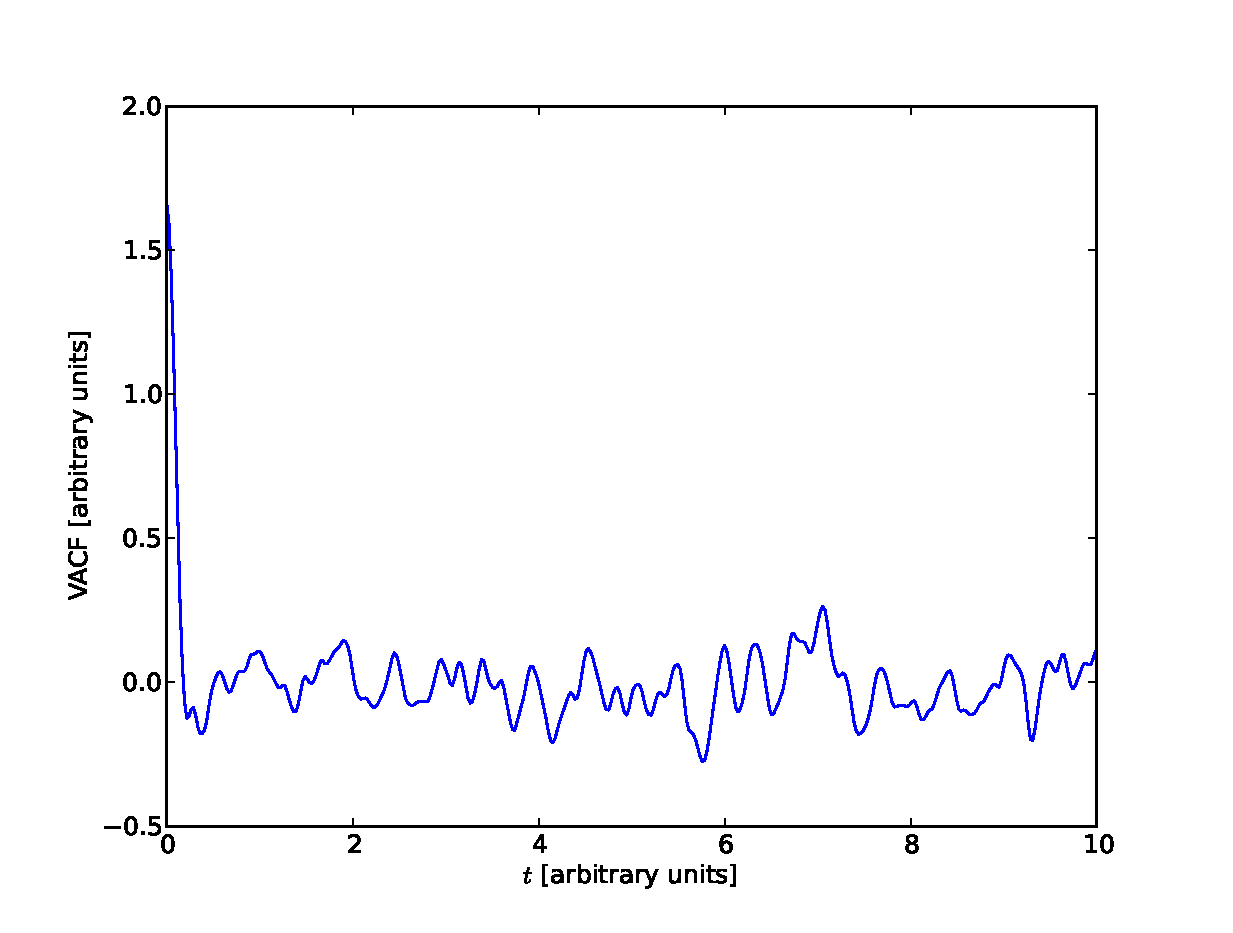
\includegraphics[width=0.35\textwidth]{vacf_time.eps}
    \label{fig:msd_time}
  }
%  \qquad % Spacing
%  \qquad % Spacing
  \subfloat[]{
    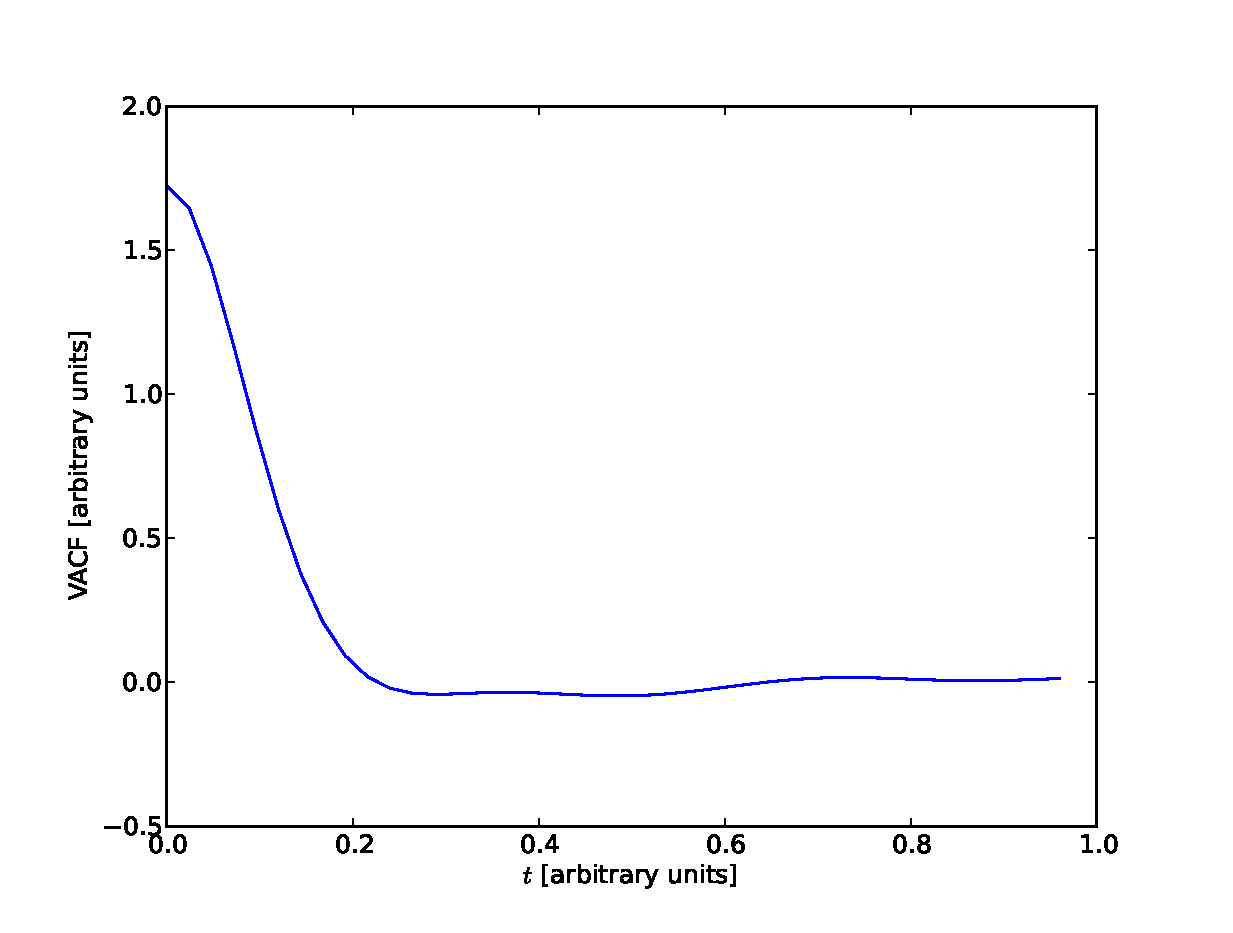
\includegraphics[width=0.35\textwidth]{vacf_time_correlated.eps}
    \label{fig:msd_time_correlated}
  }
  \caption{
    (a) Uncorrelated VACF vs time.
    (b) VACF after the correlation function has been done.
  }
\end{figure}




\newpage
\section{Assignment}

The assignment is to create a python simulation that calculates 
the diffusion coefficient from MSD and VACF, and simulate
the coefficient over different variables.

\subsection{Simulation Setup}

First part is to setup the simulation to calculate $D$.
To make it easy to start we have split the setup into
small manageable steps. An example for starting variables is

\begin{lstlisting}
n_particles = 108
temperature = 0.5
rho = 0.7
equlib_steps = 10000
n_steps = 10000
sample_freq = 24
dt = 0.001
\end{lstlisting}

\begin{enumerate}

    \item Define a sample frequency and save
    a list of position matrices \code{R} during the
    Velo-Verlet simulation, by finishing the \code{simulation}
    function.

    \item Create a function that calculates the MSD
    between two coordinate matrices \code{R}.

    \item Calculate MSD for each sampled \code{R} and
    plot MSD vs. simulation time.
    If you use the constants above it should look similar
    too figure \ref{fig:msd_time}.

    \item Implement the correlation function method
    for MSD and plot MSD vs. time.
    If you use the constants above it should look similar
    too figure \ref{fig:msd_time_correlated}.

    \item Use the correlated MSD list and
    the method for calculating the limit of MSD
    to calculate the diffusion coefficient.

    \item Follow the same procedure for calculating
    the diffusion coefficient with the VACF method.

\end{enumerate}

\textbf{Hint:} If you run your program with the settings suggested above, you will get $D \approx 0.05$.

\begin{figure}[htb]
	\centering
  \subfloat[]{
    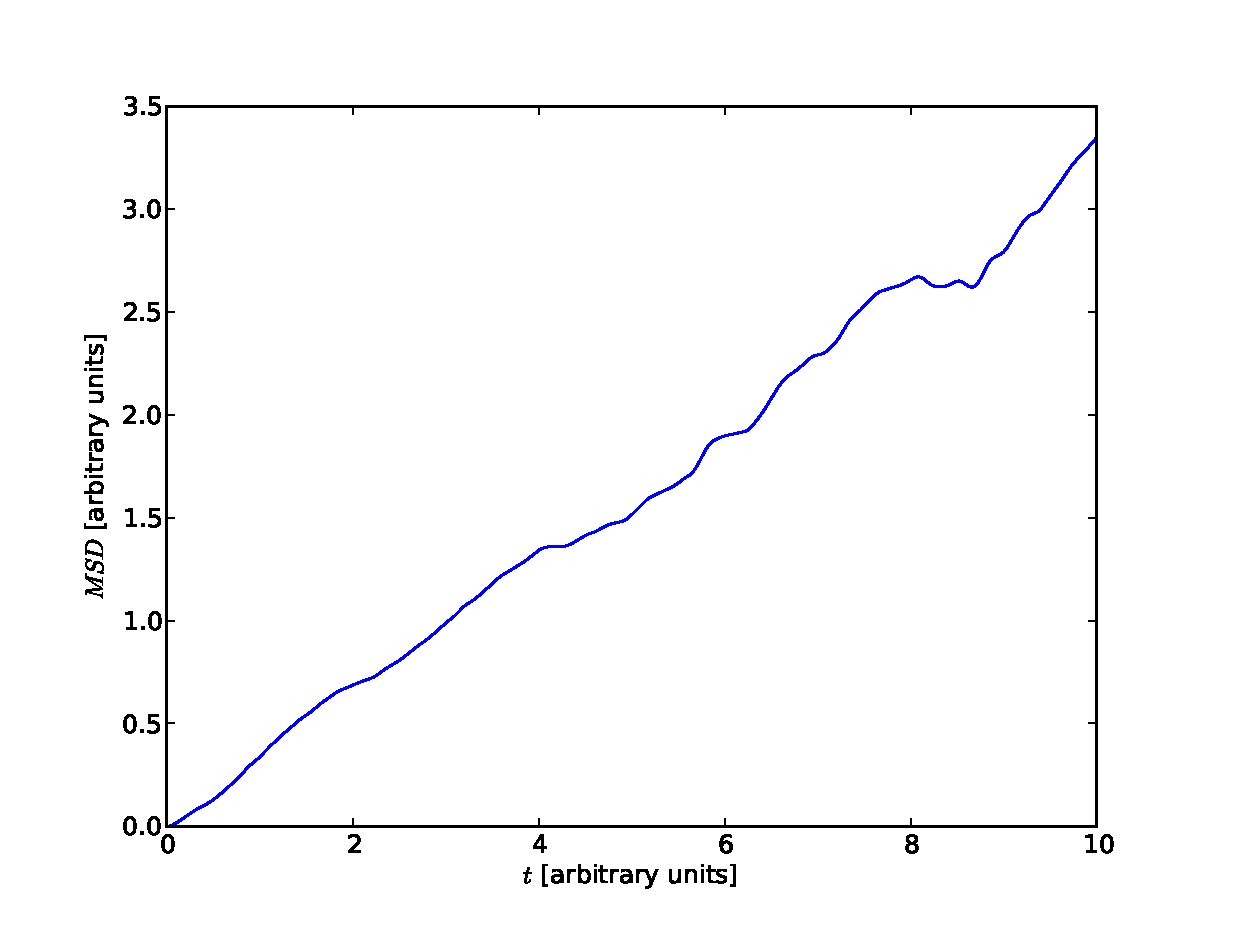
\includegraphics[width=0.5\textwidth]{msd_time.eps}
    \label{fig:msd_time}
  }
%  \qquad % Spacing
%  \qquad % Spacing
  \subfloat[]{
    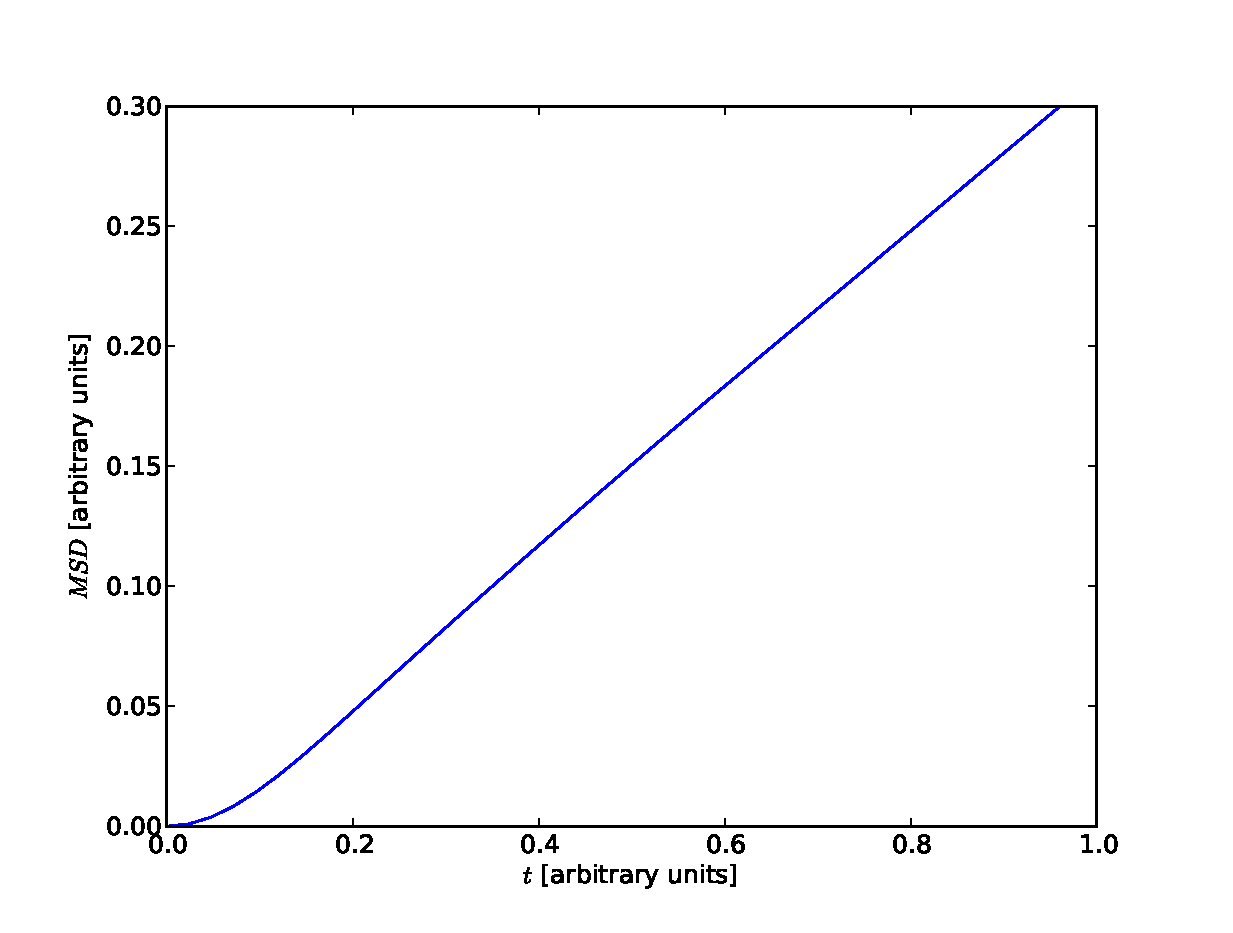
\includegraphics[width=0.5\textwidth]{msd_time_correlated.eps}
    \label{fig:msd_time_correlated}
  }
  \caption{
    (a) Uncorrelated MSD vs time.
    (b) MSD after the correlation function has been done.
  }
\end{figure}

\clearpage
\newpage
\subsection{Simulations}

Now that you have a working simulation it is time to do
some science.
You need to do the following six simulations and conclude
on the results (with plots).

\begin{itemize}
    \item {\bf Simulation 1}\newline
    Check the convergence of the diffusion coefficient
    with simulation step number.

    \item {\bf Simulation 2}\newline
    Check the convergence of the diffusion coefficient
    with system size (particle numbers)

    \item {\bf Simulation 3}\newline
    Check MSD/VACF over time for given temperature at different densities.

    \item {\bf Simulation 4}\newline
    Check MSD/VACF over time for a given density $\rho$ at different temperatures.

    \item {\bf Simulation 5}\newline
    Check the diffusion coefficient for a given temperature for different densities.

    \item {\bf Simulation 6}\newline
    Check the diffusion coefficient for a given density $\rho$ for different temperatures.

\end{itemize}



% ***************************************************
% END DOCUMENT
% ***************************************************

\end{document}

